%% Requires compilation with XeLaTeX or LuaLaTeX
\documentclass[10pt,xcolor={table,dvipsnames},t]{beamer}
\usetheme{UCBerkeley}
\usepackage{animate}

\title[SMACC]{SMACC}
\subtitle{SDSS MOC4 Asteroid Color Classification}
\author{Ben Montgomery}
\institute{University of Southern Maine}
\date{\today}

\begin{document}

\begin{frame}
  \titlepage
  % That's right, this is the SMACC talk.
\end{frame}

\section{Introduction}

\begin{frame}{From Last Time...}
\begin{itemize}
    \item The Sloan Digital Sky Survey is a multi-spectral survey of celestial objects, most notably of asteroids.
    \item Records the UGRIZ color bands.
    \item Has 471,569 observations in it.
    \item Assorted people thought there were 2, 4, and 16 distinct asteroid compositions in the SDSS.
    \item Carvano \cite{Carvano} made that 16 class claim, so I'm trying to check his results using unsupervised learning.
\end{itemize}
\end{frame}

% ------- METHODS SLIDE ----------

% 1.
\begin{frame}{Methods}
\begin{itemize}
    \item Do the same data corrections that Carvano did.
\end{itemize}
\end{frame}

% 2.
\begin{frame}{Methods}
\begin{itemize}
    \item Do the same data corrections that Carvano did.
    \item Apply the K-Means, K-Medoids, HDBSCAN*, and Agglomerative unsupervised clustering algorithms to come up with a classification scheme.
\end{itemize}
\end{frame}

% 3.
\begin{frame}{Methods}
\begin{itemize}
    \item Do the same data corrections that Carvano did.
    \item Apply the K-Means, K-Medoids, HDBSCAN*, and Agglomerative unsupervised clustering algorithms to come up with a classification scheme.
    \item Determine how good the classifications are.
\end{itemize}
\end{frame}

% 4.
\begin{frame}{Methods}
\begin{itemize}
    \item Do the same data corrections that Carvano did.
    \item Apply the K-Means, K-Medoids, HDBSCAN*, and Agglomerative unsupervised clustering algorithms to come up with a classification scheme.
    \item Determine how good the classifications are.
    \item ???
    \item Profit.
\end{itemize}
\end{frame}

\begin{frame}{Data Correction}
\begin{itemize}
Carvano's corrections were limited to removing solar contribution from the color data. in an error-correcting manner.

For the $i^{th}$ band $\lambda_{i}$ in UGRIZ, the reflectance color is calculated as
$$
C_{\lambda_{i}} = -2.5\left(\log_{10}R_{\lambda_i} + \log_{10}R_{\lambda_{ref}} \right)
$$
in order to produce the color reflectance gradient 
$$
\gamma_{j} = -0.4\dfrac{C_{\lambda_{i + 1}} - C_{\lambda_{i}}}{\lambda_{i + 1} - \lambda_{i}}
$$
First downside: only four columns to make predictions from.
\end{itemize}
\end{frame}


\begin{frame}{Data Correction}
% Phase reddening has the same effect as a Doppler shift. Instead of sound appearing to change, colors appear to change.
\vspace*{\fill}
There is all kinds of error in the SDSS, such as phase reddening and zenith-induced error. It is expected that not correcting for these factors will produce significantly errant results \cite{sanchez, hm_gmode}.
\vspace*{\fill}
% In other words, everything is going to go south really quickly.
\end{frame}

\begin{frame}{Visualizing Carvano's Classifications}
% Each distinct color represents a class. The PCA plot isn't encouraging; the data should not be linearly seperable. This may suggest that Carvano's corrections only preserve brightness, which is a huge problem. That isn't a meaningful metric.
\begin{figure*}
\begin{center}
    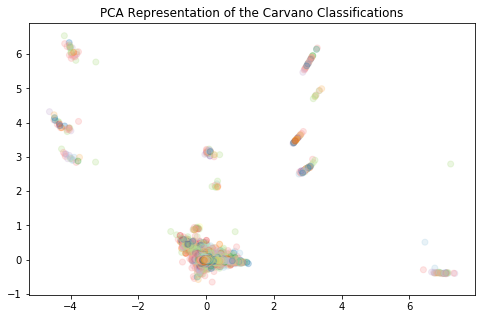
\includegraphics[width=0.5\textwidth]{images/carvano_pca.png}
    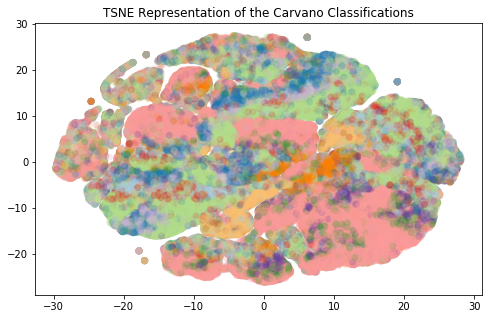
\includegraphics[width=0.5\textwidth]{images/carvano_tsne.png}
\end{center}
\end{figure*}
\end{frame}

\begin{frame}
\begin{figure*}
\topskip0pt
\vspace*{9em}
\Huge \textbf{K-Means++}
\hline
\vspace*{\fill}
\end{figure*}
\end{frame}

\begin{frame}{Applying K-Means++}
% First is K-Means. Elbow is below. There is a closed-form equation which states the elbow is 9, and from the graph, that looks pretty reasonable.
% K-means is used as a heuristic, as the SDSS has a lot of noise in it; k-means is highly influenced by outliers.
\begin{figure*}
\begin{center}
    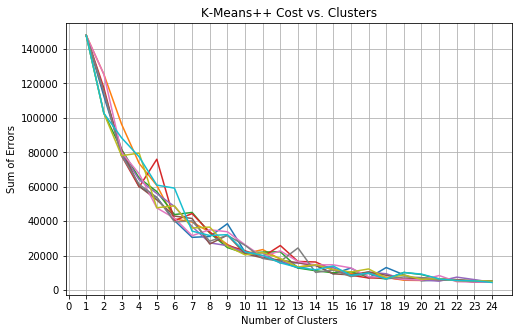
\includegraphics[width=0.7\textwidth]{images/kmeans-elbow.png}
\end{center}
\end{figure*}
\end{frame}

\begin{frame}{Applying K-Means++}
\begin{figure*}
\begin{center}
    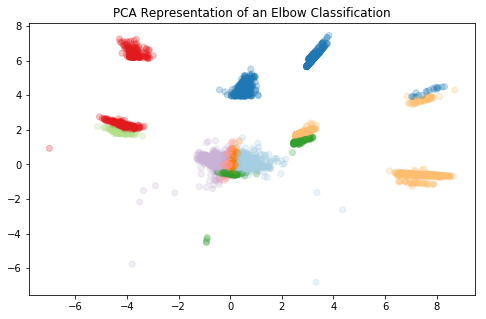
\includegraphics[width=0.5\textwidth]{images/kmeans-pca.png}
    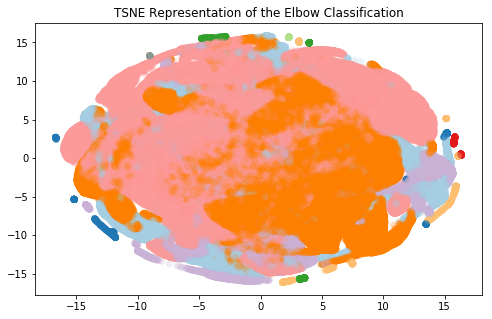
\includegraphics[width=0.5\textwidth]{images/kmeans-tsne.png}
\end{center}
\end{figure*}
\end{frame}

\begin{frame}
\begin{figure*}
\topskip0pt
\vspace*{9em}
\Huge \textbf{K-Medoids}
\hline
\vspace*{\fill}
\end{figure*}
\end{frame}

\begin{frame}{Applying K-Mediods}
\begin{figure*}
\begin{center}
    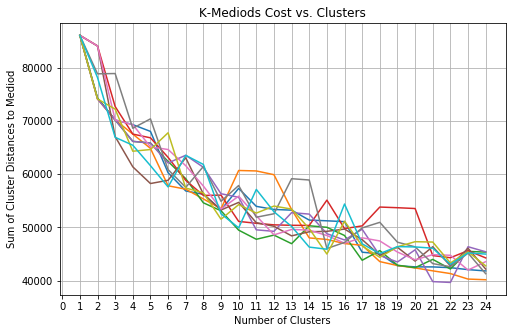
\includegraphics[width=0.7\textwidth]{images/kmed-cost.png}
\end{center}
\end{figure*}
\end{frame}

\begin{frame}{Applying K-Mediods}
\begin{figure*}
\begin{center}
    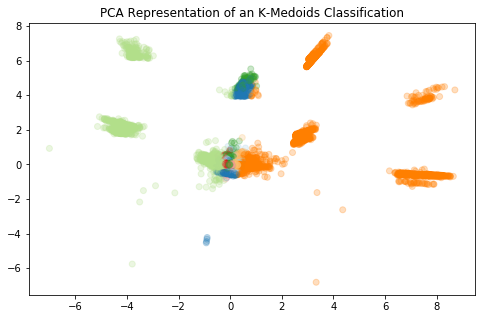
\includegraphics[width=0.5\textwidth]{images/kmed_pca.png}
    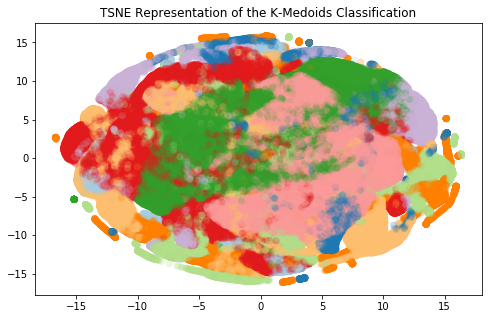
\includegraphics[width=0.5\textwidth]{images/kmed_tsne.png}
\end{center}
\end{figure*}
\end{frame}

\begin{frame}
\begin{figure*}
\topskip0pt
\vspace*{9em}
\Huge \textbf{HDBSCAN*}
\hline
\vspace*{\fill}
\end{figure*}
\end{frame}

\begin{frame}{Applying HDBSCAN*}
\begin{figure*}
\begin{center}
    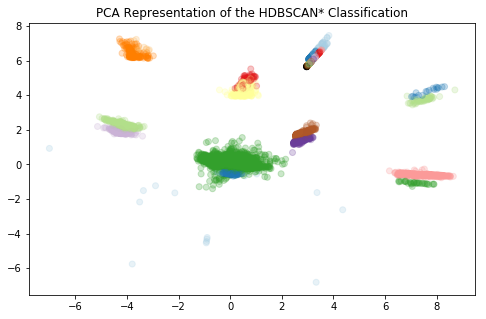
\includegraphics[width=0.7\textwidth]{images/hdbscan_pca.png}
\end{center}
\end{figure*}
\end{frame}

\begin{frame}
\begin{figure*}
\topskip0pt
\vspace*{9em}
    \Huge \textbf{Agglomerative} \\
    \Huge \textbf{Clustering}
    \hline
\vspace*{\fill}
\end{figure*}
\end{frame}

\begin{frame}{Applying Agglomerative Clustering}
\begin{figure*}
\begin{center}
    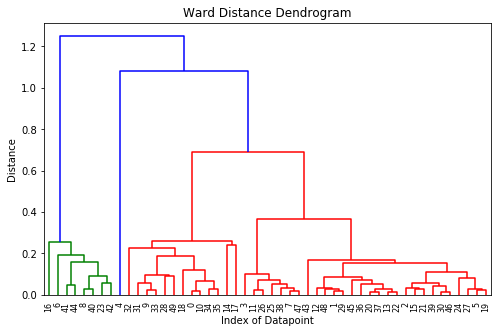
\includegraphics[width=0.7\textwidth]{images/dendrogram.png}
\end{center}
\end{figure*}
\end{frame}

\begin{frame}{Applying Agglomerative Clustering}
\begin{figure*}
\begin{center}
    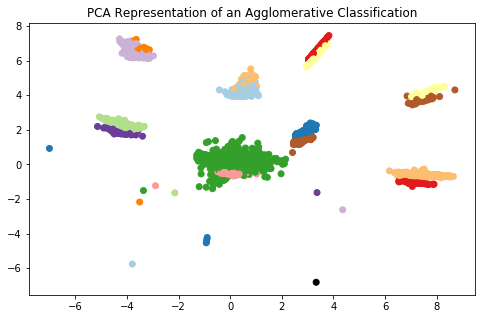
\includegraphics[width=0.7\textwidth]{images/agglomerative_pca.png}
\end{center}
\end{figure*}
\end{frame}

\begin{frame}{How Good are the Results?}
For a given asteroid $a$ out of $n$ total, having $m_a$ observations, and the number of class occurrences $c1_a, c2_a ... cn_a$ for a given classification $cn$, consistency will be defined as:
$$
\sum_{a=0}^n \dfrac{max(c1_a, c2_a ... cn_a)}{m_a}
$$
\begin{tabular}{c | c | c | c | c}
     & K-Means++ & K-Medoids & HDBSCAN* & Agglomerative\\
     \hline
     Consistency & 87.8\% & 77.3\% & 97.2\% & 99.8\%\\
     Blind-Guess & 60.0\% & 25.7\% & 97.2\% & 99.3\%\\
     \# Classes  & 9      & ~9     & 0 - 3000+ (14) &  9
\end{tabular}
\end{frame}

\begin{frame}{How Good are the Results?}
\begin{figure*}
\begin{center}
    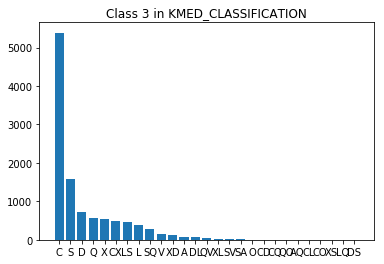
\includegraphics[width=0.5\textwidth]{images/bar-sample.png}
    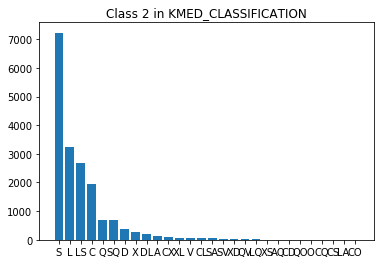
\includegraphics[width=0.5\textwidth]{images/bar-sample-2.png}
\end{center}
\end{figure*}
\end{frame}

\begin{frame}
\begin{figure*}
\vspace{-2em}
\begin{center}
    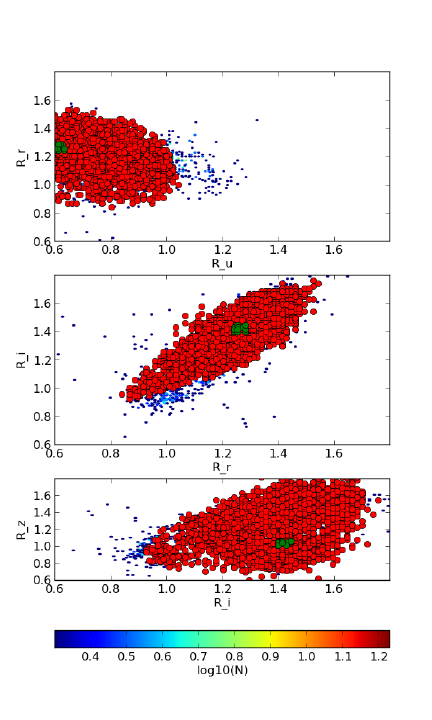
\includegraphics[height=1.2\textheight]{images/gmode.png}
\end{center}
\end{figure*}
\end{frame}

\begin{frame}
\frametitle{References}

\bibliographystyle{IEEEtran}
\bibliography{references}

\end{frame}


\end{document}
